\section{Data}

Some pre-analysis result of the data


In the report (looking for some report), the penetration of mobile device is XXX, almost every XX people got a Mobile Phone in the urban. XX. As Figure~\ref{fig:data_over} shows, multiple social characteristics of a people is sampled, including income, education, etc. 

\begin{figure}[htb!]
 \centering % avoid the use of \begin{center}...\end{center} and use \centering instead (more compact)
 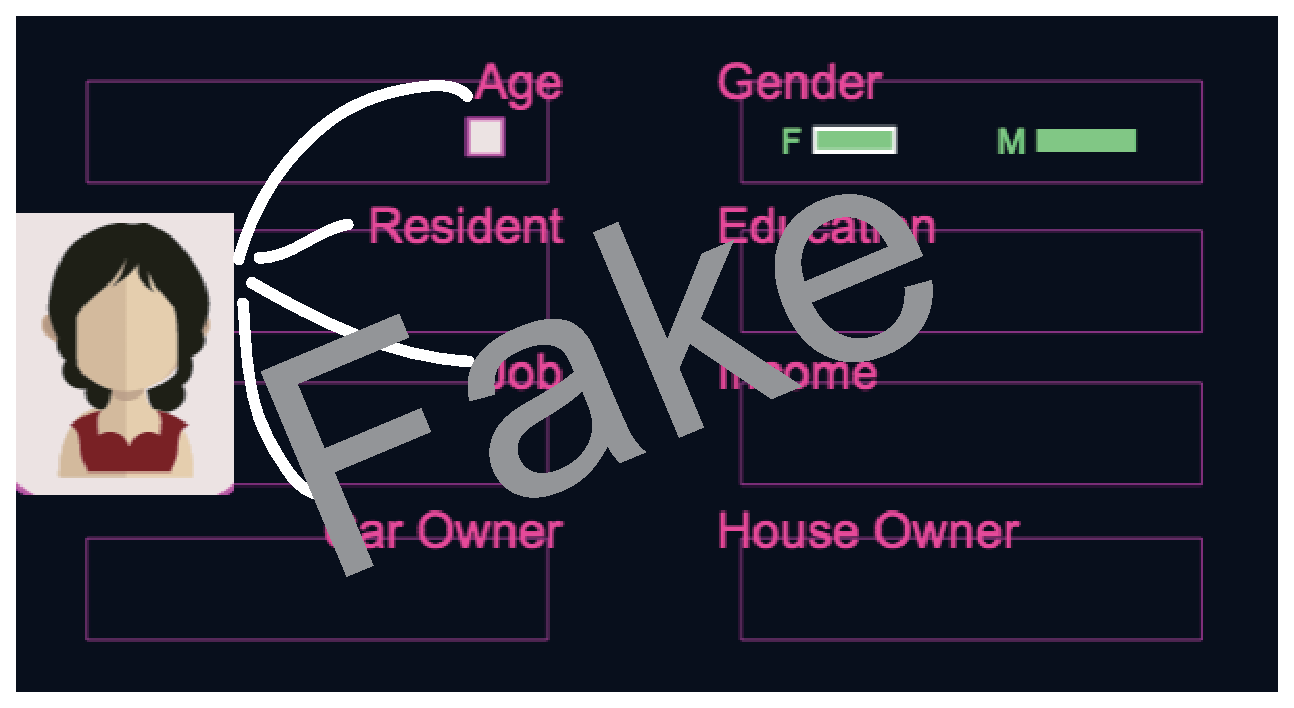
\includegraphics[width=\columnwidth]{pictures/data_over1}
 \caption{Overview of Social Characteristics}
 \label{fig:data_over}
\end{figure}

The coverage of the data in spatial and social aspects. The distribution of age is consistent to the traditional survey (Shenzhen Census?).... Figure~\ref{fig:data_stat} shows...


\begin{figure}[htb!]
 \centering % avoid the use of \begin{center}...\end{center} and use \centering instead (more compact)
 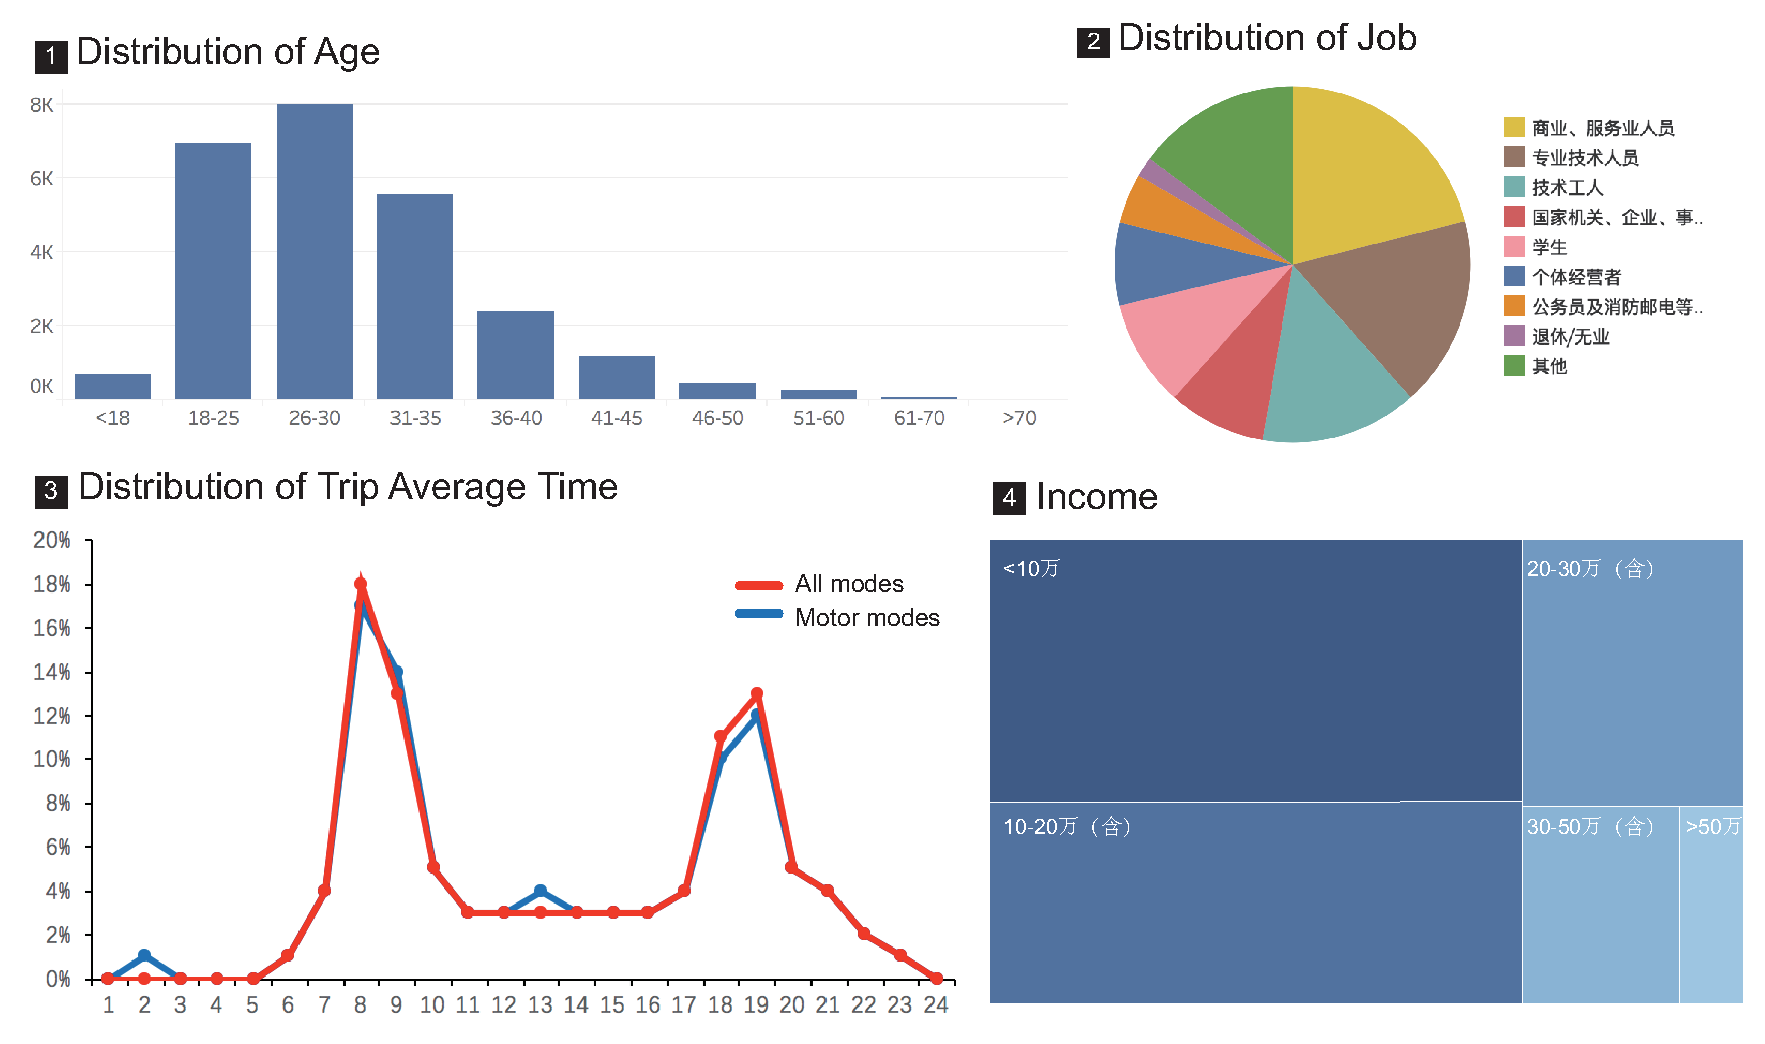
\includegraphics[width=\columnwidth]{pictures/data_detail}
 \caption{Statistics}
 \label{fig:data_stat}
\end{figure}